% !TeX root = RJwrapper.tex
\title{xyz: a greate package that I created}
\author{by Author One and Author Two}

\maketitle

\abstract{%
An abstract of less than 150 words.
}

\hypertarget{introduction}{%
\section{Introduction}\label{introduction}}

An introduction to the paper \ldots{}

\hypertarget{another-section-that-needs-to-be-in-the-sentence-case}{%
\section{Another section (\ldots{} that needs to be in the sentence
case)}\label{another-section-that-needs-to-be-in-the-sentence-case}}

There will likely be several sections, including literature review with
some references in the \texttt{.bib} file, some user case demos with
code snippets as follows:

\begin{Schunk}
\begin{Sinput}
x <- 1:10
plot(x)
\end{Sinput}
\end{Schunk}

and a plot with cross-reference and captions as in Figure
@ref(fig:myplot),

\begin{Schunk}
\begin{figure}
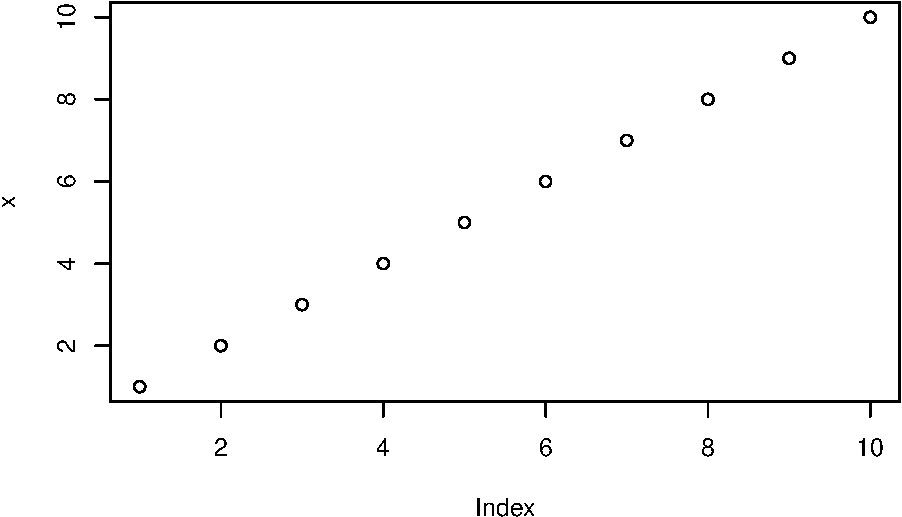
\includegraphics{sample-article_files/figure-latex/myplot-1} \caption[A caption should include three elements]{A caption should include three elements: 1) a one sentence summary of what the plot is about; 2) the details of elements being plotted; and 3) the messages from the plot.}\label{fig:myplot}
\end{figure}
\end{Schunk}

\hypertarget{summary}{%
\subsection{Summary}\label{summary}}

This file is only a basic article template. For full details of
\emph{The R Journal} style and information on how to prepare your
article for submission, see the
\href{https://journal.r-project.org/share/author-guide.pdf}{Instructions
for Authors}.

\bibliography{sample-article.bib}

\address{%
Author One\\
Affiliation\\%
line 1\\ line 2\\
%
\url{https://journal.r-project.org}%
\\\textit{ORCiD: \href{https://orcid.org/0000-0002-9079-593X}{0000-0002-9079-593X}}%
\\\href{mailto:author1@work}{\nolinkurl{author1@work}}
}

\address{%
Author Two\\
Affiliation 1\\%
line 1 affiliation 1\\ line 2 affiliation 1\\
Affiliation 2\\%
line 1 affiliation 2\\ line 2 affiliation 2\\
%
\url{https://journal.r-project.org}%
\\\textit{ORCiD: \href{https://orcid.org/0000-0002-9079-593X}{0000-0002-9079-593X}}%
\\\href{mailto:author2@work}{\nolinkurl{author2@work}}
}
